\chapter{Directional Derivatives and Gradient Vector}

\section{Directional Derivatives}
\begin{definition}
    The \textbf{directional derivative} of $f$ at $(x_0, y_0) $ in the direction of a unit vector $\textbf{u}=<a, b>$ is
    \begin{equation}
        D_uf(x_0, y_0)= \lim_{h \to 0} \frac{f(x_0 + ha, y_0 + hb) - f(x_0, y_0}{h}
    \end{equation}
    if this limit exists.
\end{definition}

\begin{figure}[h]
    \centering
    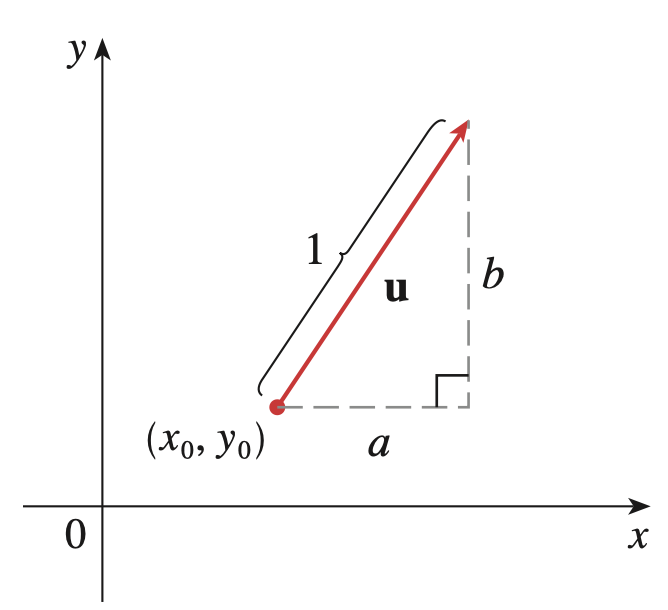
\includegraphics[scale=0.6]{chapter002/figures/fig002}
    \caption{Unit Vector}
    \label{fig:Unit Vector}
\end{figure}

\begin{figure}[h]
    \centering
    \cite{calculus}
    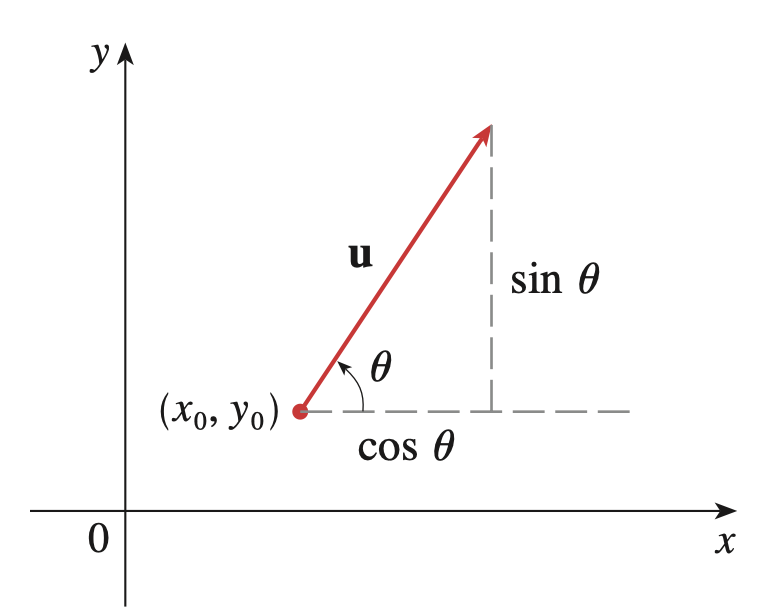
\includegraphics[scale=0.6]{chapter002/figures/fig003}
    \caption{Unit Vector}
    \label{fig:Unit Vector}
\end{figure}

\begin{figure}[h]
    \centering
    \cite{calculus}
    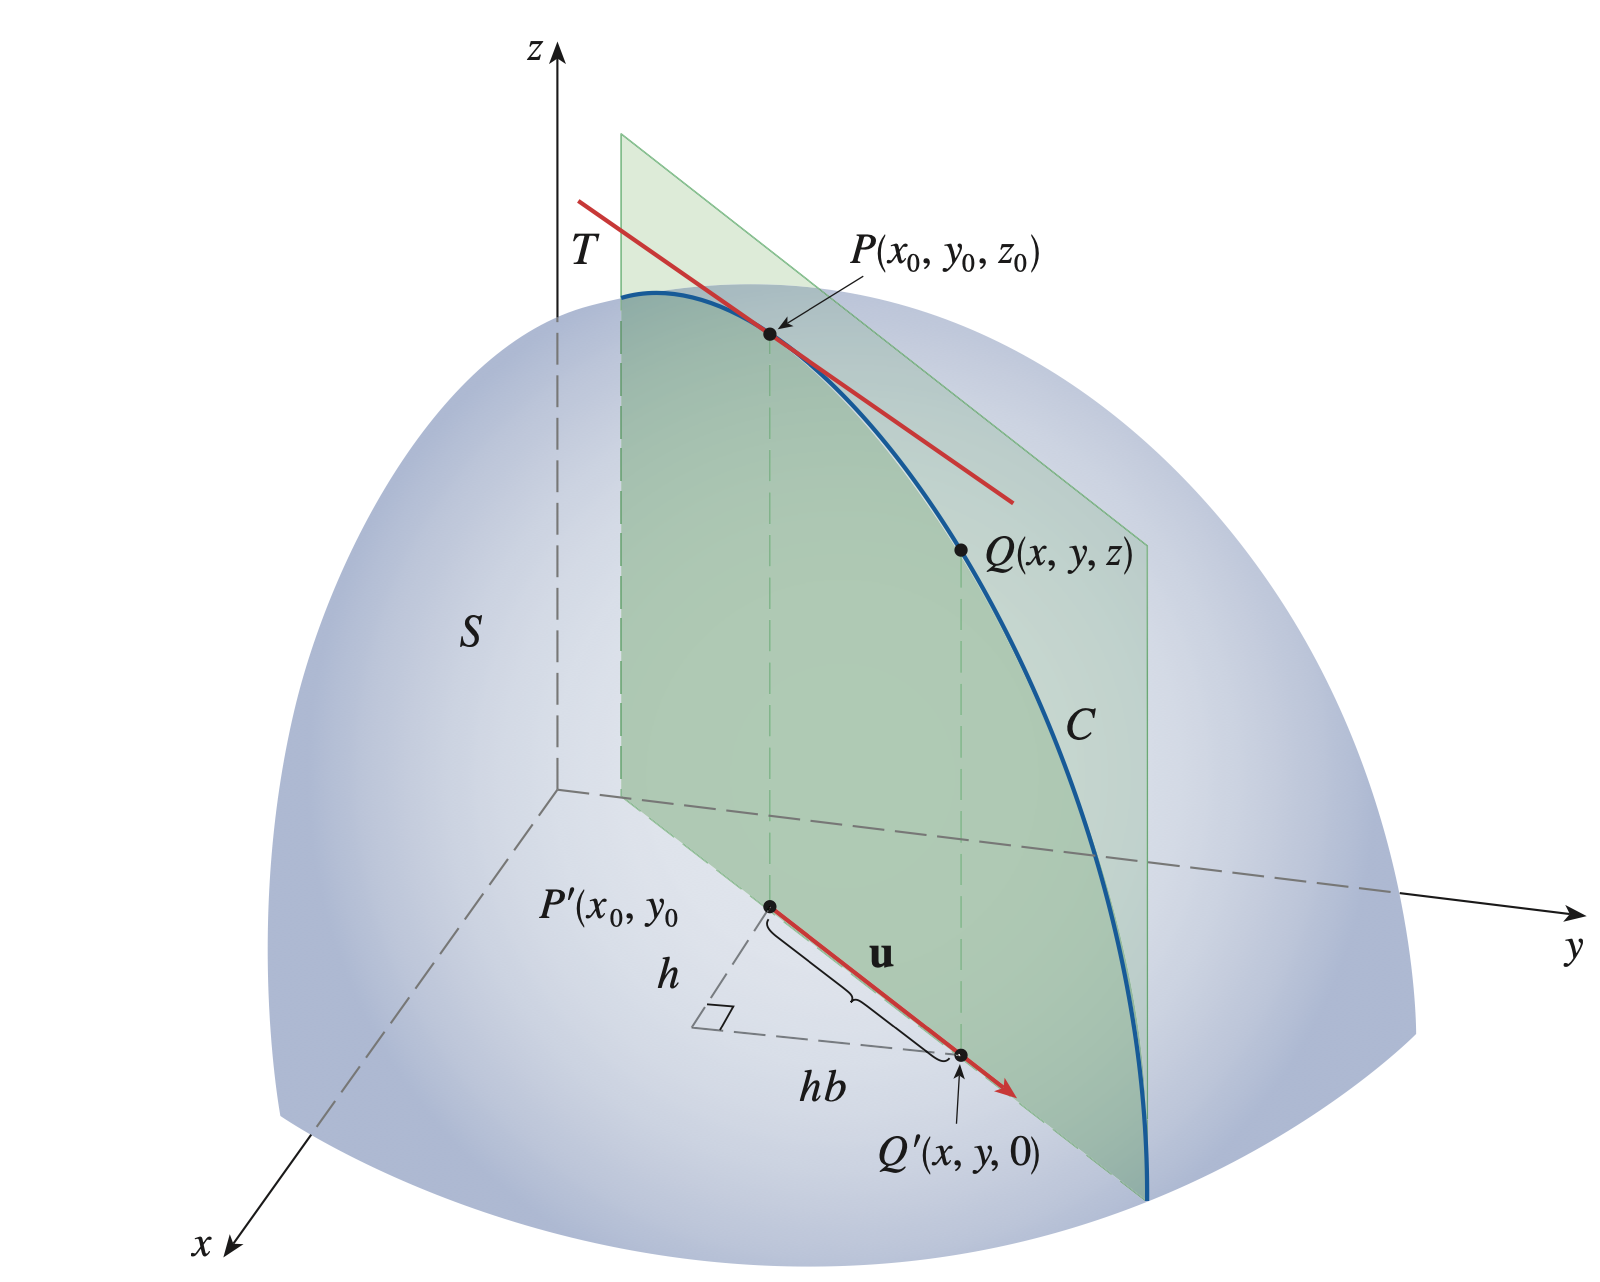
\includegraphics[scale=0.5]{chapter002/figures/fig001}
    \caption{Directional Derivative}
    \label{fig:Directional Derivative}
\end{figure}

\begin{theorem}
    If $f$ is a differentiable function of $x$ and $y$, then $f$ has a directional derivative in the direction of any unit vector $\textbf{u} = <a, b>$ and
    \begin{equation}
        D_uf(x, y) = f_x(x, y)a + f_y(x, y)b
    \end{equation}
\end{theorem}

\subsubsection{Proof}
If we define a function $g$ of the single variable $h$ by
$$
    g(h) = f(x_0 + ha, y_0 + hb)
$$
then, by the definition of a derivative, we have
$$
    g'(0) = \lim_{h \to 0}\frac{g(h) - g(0)}{h} = \lim_{h \to 0}\frac{f(x_0 + ha, y_0 + hb) - f(x_0, y_0)}{h} = D_uf(x_0, y_0)
$$
let,

\begin{tabularx}{\linewidth}{@{}XX@{}}
    $
        x = x_0 + ha
    $
    &
    $
        y = y_0 + hb
    $
\end{tabularx}

thus,
$$
    g(h) = f(x, y)
$$
$$
    g'(h) = \frac{\partial f}{\partial x}\frac{\partial x}{\partial h} + \frac{\partial f}{\partial y}\frac{\partial y}{\partial h} = f_x(x, y)a + f_y(x, y)b
$$
since,

\begin{tabularx}{\linewidth}{@{}XX@{}}
$$
    \frac{\partial x}{\partial h}=\frac{\partial (x_0 + ha)}{\partial h}=a
$$
&
$$
    \frac{\partial y}{\partial h}=\frac{\partial (y_0 + hb)}{\partial h}=b
$$
\end{tabularx}

\begin{theorem}
    If the unit vector $\textbf{u}$ makes an angle $\theta$ with the positive x-axis, then we can write $\textbf{u}=<\cos \theta, \sin \theta>$, then
    \begin{equation}
        \label{eq:Directional Derivative}
        D_uf(x, y)=f_x(x, y)\cos \theta + f_y(x, y) \sin \theta
    \end{equation}
\end{theorem}

\section{The Gradient Vector}
\begin{definition}
    The directional derivative of a differentiable function can be written as the dot product of two vectors.
    \begin{equation}
        D_uf(x, y)=f_x(x, y)a + f_y(x, y)b=<f_x(x, y), f_y(x, y)> \cdot <a, b> = <f_x(x, y), f_y(x, y)> \cdot u
    \end{equation}
\end{definition}
$<f_x(x, y), f_y(x, y)>$ is called gradient vector and noted as $\nabla f$

\subsection{Example 1}
Find the directional derivative of the function $f(x, y)=x^2y^3-4y$ at the point $(2, -1)$ in the direction of the vector $\vec{v}=2\vec{i} + 5\vec{j}$

\subsubsection{Solution}
$$
    \nabla f(x, y)=<f_x(x, y), f_y(x, y)>=<2xy^3, 3x^2y^2 - 4>
$$
$$
    \nabla f(2, -1)=<-4, 8>
$$
Note that $v$ is not a unit vector, but since $|\vec{v}|=\sqrt{29}$, the unit vector in the direction of $\vec{v}$ is
$$
    \vec{u}=\frac{\vec{v}}{|\vec{v}|}=\frac{2}{\sqrt{29}}\vec{i} + \frac{5}{\sqrt{29}}\vec{j}
$$
Therefore, we have
$$
    D_uf(2, -1)=\nabla f(2, -1) \cdot \vec{u} = (-4 \vec{i} + 8 \vec{j}) \cdot (\frac{2}{\sqrt{29}}\vec{i} + \frac{5}{\sqrt{29}}\vec{j})=\frac{-4 \cdot 2 + 8 \cdot 5}{\sqrt{29}} = \frac{32}{\sqrt{29}}
$$

\begin{figure}[h]
    \centering
    \cite{calculus}
    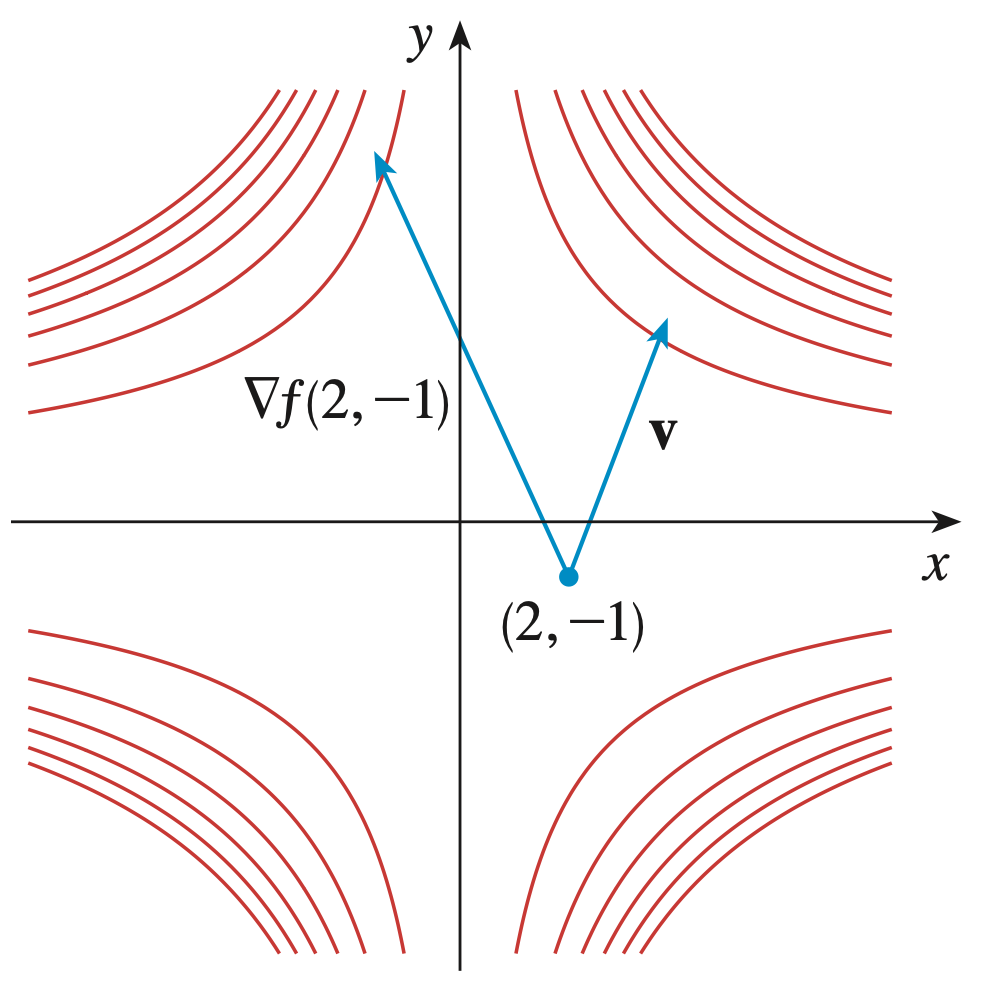
\includegraphics[scale=0.6]{chapter002/figures/fig004}
    \caption{Gradient Vector}
    \label{fig:Gradient Vector}
\end{figure}

\section{Maximizing the Directional Derivative}

\begin{theorem}
    Suppose $f$ is a differentiable function of two or three variables. The maximum value of the directional derivative $D_uf(x)$ is $| \nabla f(x)|$ and it occurs when $\vec{u}$ has the same direction as the gradient vector $\nabla f(x)$
\end{theorem}
\subsubsection{Proof}
\begin{equation}
    D_uf=\nabla f \cdot \vec{u}=|\nabla f||\vec{u}|\cos \theta = |\nabla f| \cos \theta
\end{equation}
where $\theta$ is the angle between $\nabla f$ and $\vec{u}$. The maximum value of $\cos \theta$ is 1 and this occurs when $\theta=0$. Therefore the maximum value of $D_uf$ is  $|\nabla f|$ and it occurs when $\theta=0$, that is, when $\vec{u}$ has the same direction as $\nabla f$.

\subsection{Example 2}
(a) If $f(x, y)=xe^y$, find the rate of change of $f$ at the point $P(2, 0)$ in the direction from $P$ to $Q(\frac{1}{2}, 2)$.
(b) In what direction does $f$ have the maximum rate of change? What is this maximum rate of change?

\subsubsection{Solution}
$$
    \nabla f(x, y)=<f_x, f_y>=<e^y, xe^y>
$$
$$
    \nabla f(2, 0)=<1, 2>
$$
(a)
The unit vector in the direction of $\vec{PQ}=<-\frac{3}{2}, 2>$ is $\vec{u}=<-\frac{3}{5}, \frac{4}{5}>$, so the rate of change of $f$ in the direction from $P$ to $Q$ is
$$
    D_uf(2, 0)=\nabla f(2, 0) \cdot \vec{u} = <1, 2> \cdot <-\frac{3}{5}, \frac{4}{5}> = 1
$$ 
(b)
$f$ increases fastest in the direction of the gradient vector $\nabla f(2, 0)=<1, 2>$. The maximum rate of change is
$$
    |\nabla f(2, 0)| = |<1, 2>| = \sqrt{5}
$$
\begin{figure}[h]
    \centering
    \cite{calculus}
    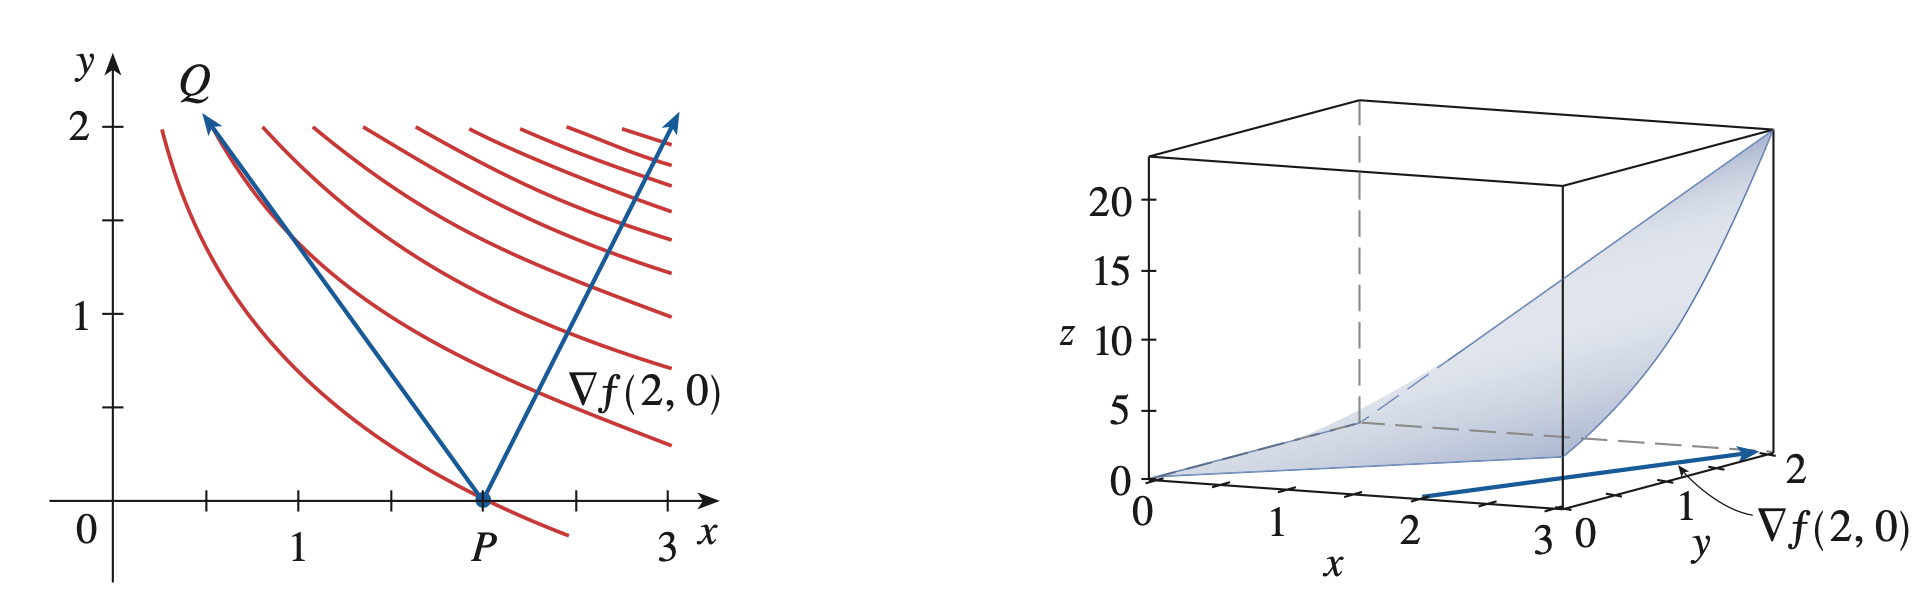
\includegraphics[scale=0.45]{chapter002/figures/fig005}
    \caption{Gradient Vector Example}
    \label{fig:Gradient Vector Example}
\end{figure}

\section{Applications}
\subsection{Snake reversals and stripes}
In a study of the survivorship of juvenile garter snakes, a researcher arrived at the model (\cite{calculus}, page 614)
$$
    F = 4.2 + 0.008R + 0.102S + 0.017R^2 - 0.034S^2 - 0.268RS
$$
where $F$ is a measure of the fitness of the snake, $R$ measures the number of reversals of direction during flight from a predator, and $S$ measures the degree of stripedness in the color pattern of the snake. How does $F$ change when $R=3$ and $S=2$ if the phenotype changes so that $R$ and $S$ increased by equal amounts?

The gradient vector of $F$ is
$$
    \nabla F(R, S) = [F_R, F_S] = [0.008 + 0.034R - 0.268S, 0.102 - 0.068S - 0.268R]
$$
and when $R=3$ and $S=2$ this becomes
$$
    \nabla F(3, 2) = [-0.426, -0.838]
$$
We want the derivative in the direction halfway between $\vec{i}$ and $\vec{j}$, that is, in the direction $\vec{v}=[1, 1]$. The unit vector in this direction is $\vec{u}=(1/\sqrt{2})[1, 1]$, so the directional derivative is
$$
    D_{\vec{u}}F(3, 2)=\nabla F(3, 2) \cdot \vec{u}=[-0.426, -0.838] \cdot [\frac{1}{\sqrt{2}}, \frac{1}{\sqrt{2}}]
    \approx 0.894
$$
This means that the fitness function at (3, 2) decreases at a rate of 0.894 units when $R$ and $S$ increase by equal amount.